\documentclass{article}
\usepackage{Sweave}
\usepackage{float}
\usepackage{graphicx}
\usepackage{natbib}
\usepackage{amsmath}
\usepackage{pdflscape}
\usepackage{hyperref}
\usepackage{indentfirst}
\usepackage[top=1.0in, bottom=1.0in, left=1.1in, right=1.1in]{geometry}
\usepackage[utf8]{inputenc}

\title{Mast-Trait}
\author{Xiaomao Wang}

\begin{document}



\section{Results}
\begin{enumerate}
\item Gathered data
\begin{enumerate}
\item Structure of data from Silvics
\begin{enumerate}

\item Angiosperm 79\% (98/124) with masting data; Strong asting and weak masting split almost equally 52\% (51/98); Gymnosperm 95\% (61/64) with masting data; almost all species are strong masting 89\% (54/61)
\end{enumerate}

\item Number of traits for different hypotheses
\begin{enumerate}
\item For angiosperm, we have data for:
\begin{enumerate}
\item Predator satiation: seed weight, fruit size, oil content, seed dispersal mode, seed dormancy
\item Pollination coupling: pollination mode, reproductive type
\item Resource matching: drought tolerance, leaf longevity
\end{enumerate}
\item For gymnosperm, we have the same data as for angiosperm, but we only have oil content for strong masting species and all the gymnosperm species are wind pollinated.
\end{enumerate}
\end{enumerate}


\newgeometry{margin=1cm}
\begin{figure}[p]
\centering
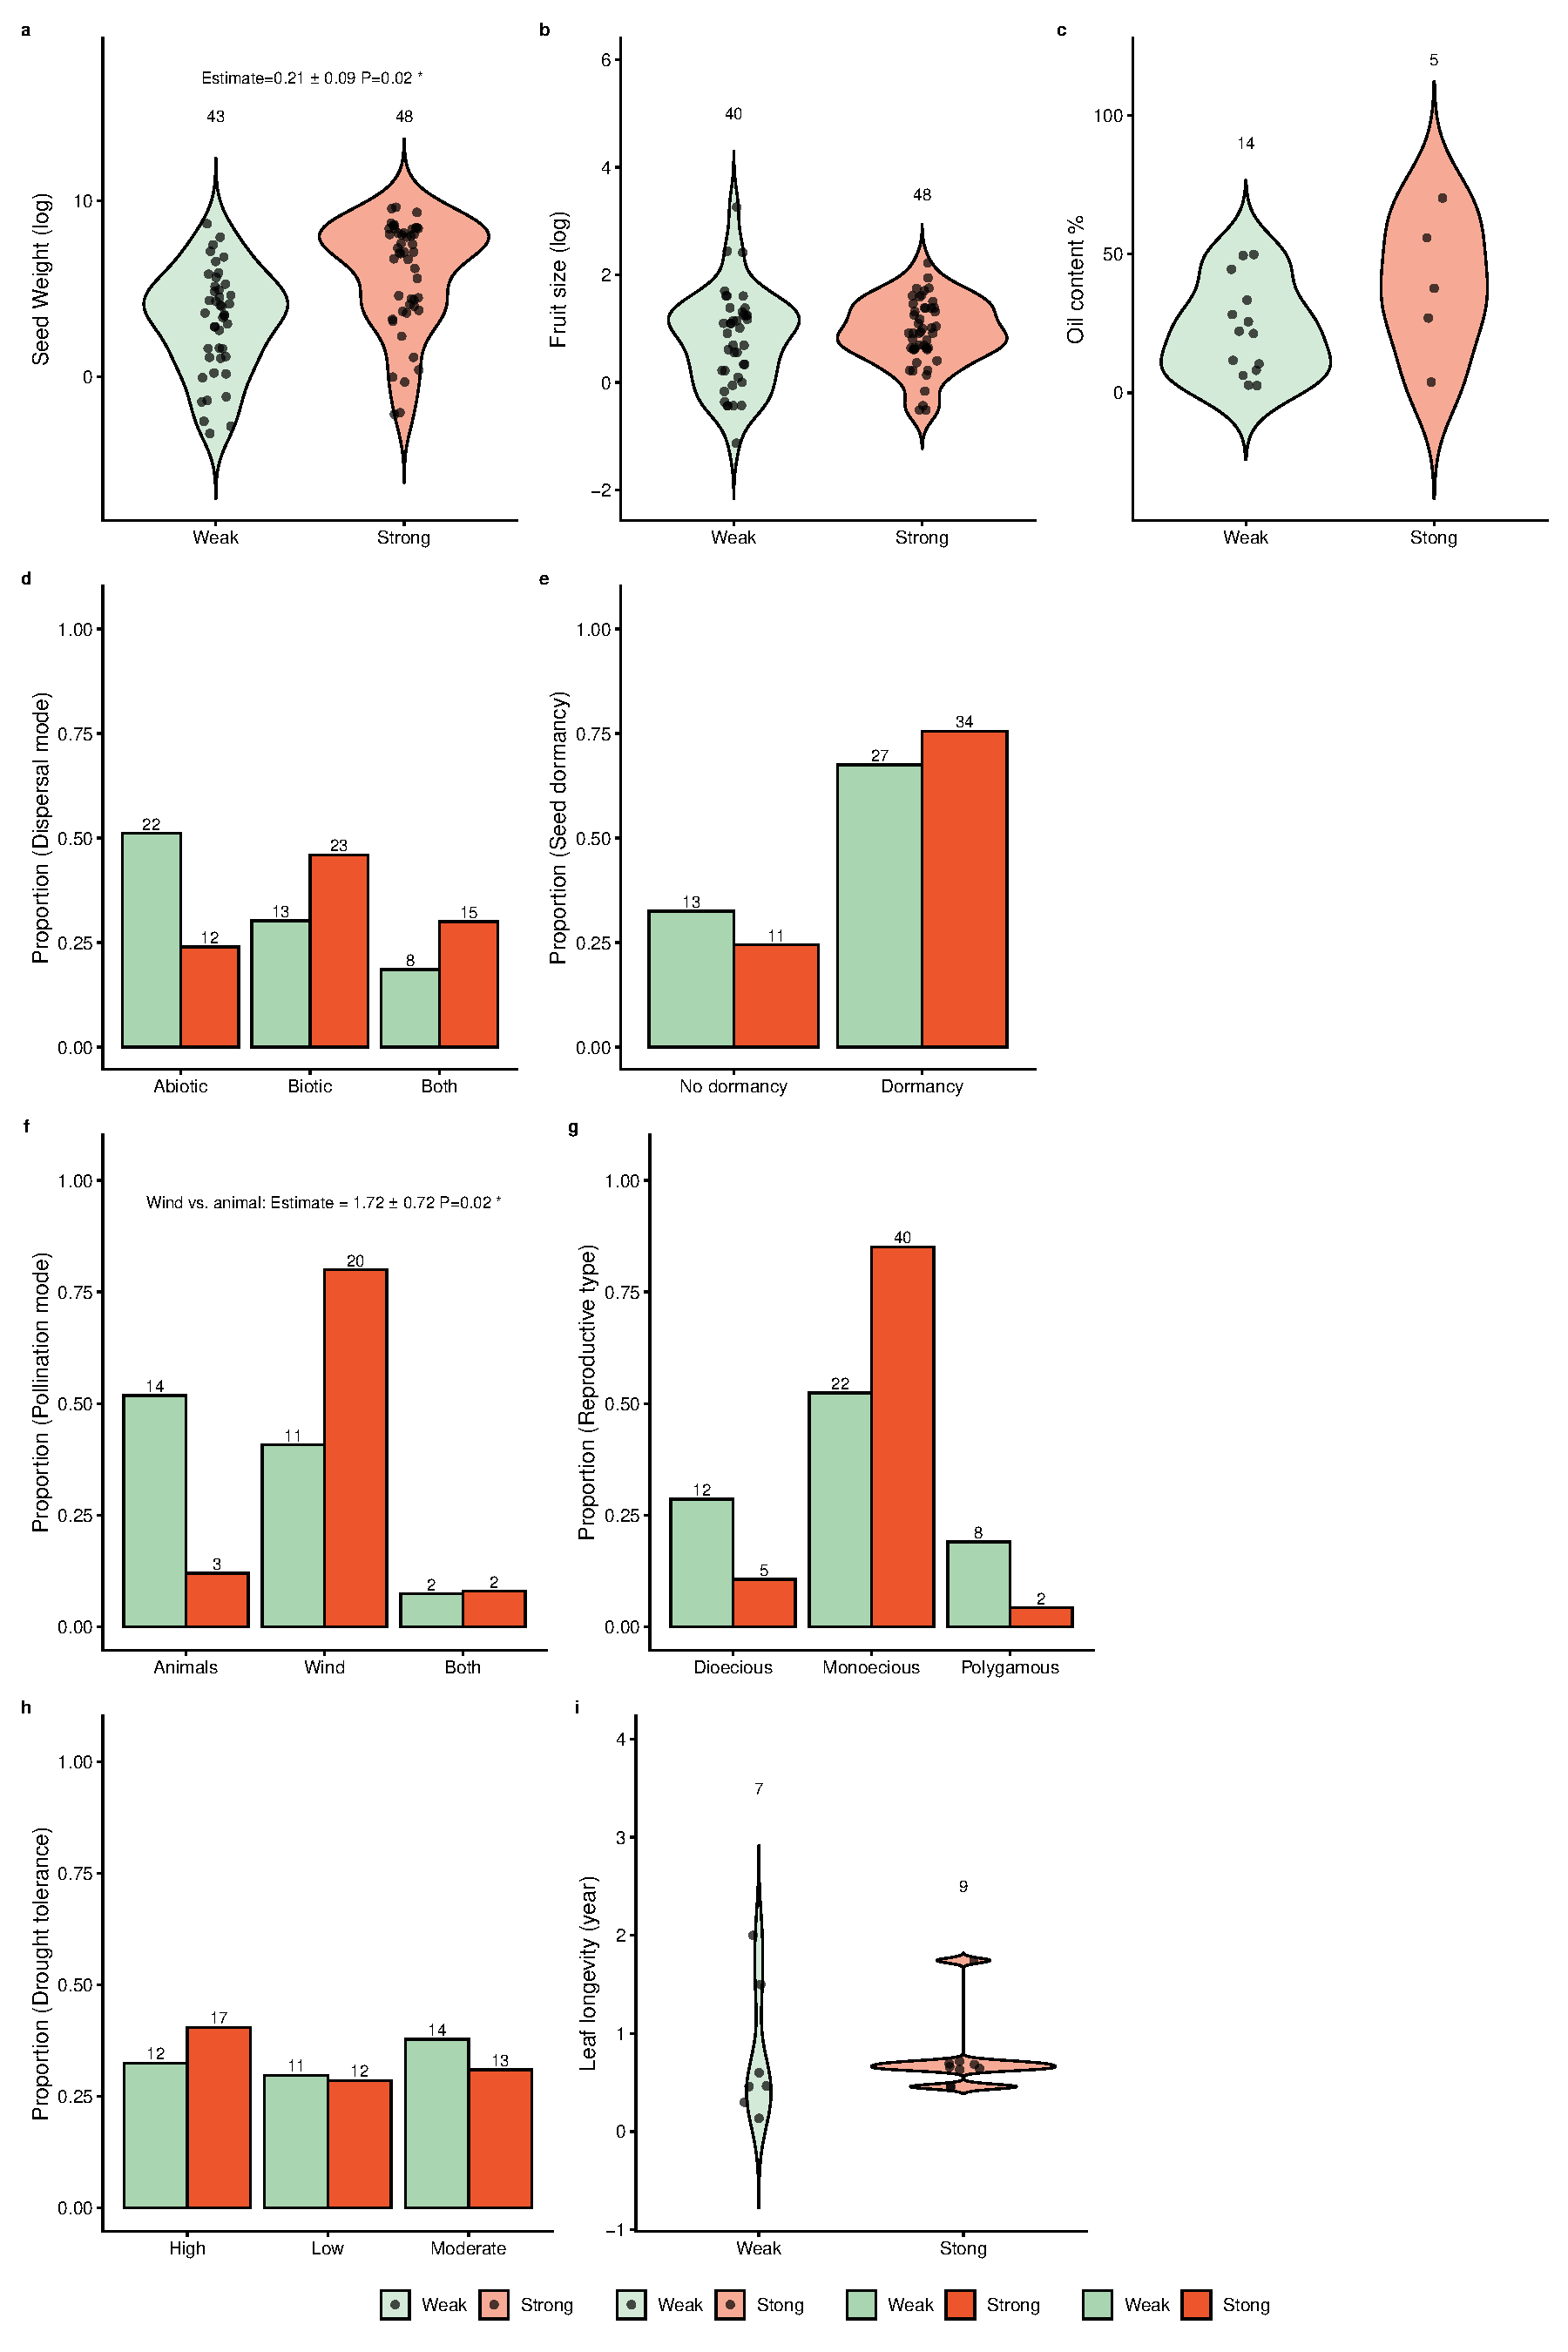
\includegraphics[width=\textwidth, height=0.8\textheight]{../output/figures/rawDataWithStatsAngio.pdf}
\caption{How plant traits related to different hypotheses differ in strong masting and weak masting for angiosperm species: We show data for traits related to the predator satiation hypothesis (a-e), pollination coupling hypothesis (f-g) and the resource matching hypothesis (h-i) as either violin plots (a-c, i) or proportional histograms (d-h) separated by species categorized as strong masting (red) or weak masting (green). We show model summaries only where significant (P-value < 0.5) and also report the model sample size (N), regression coefficient (Estimate), and phylogenetic signal parameter $\alpha$. Full model results are show in Table \ref{tab:regressionangio}.}
\label{fig:rawangio}
\end{figure}

\begin{figure}[p]
\centering
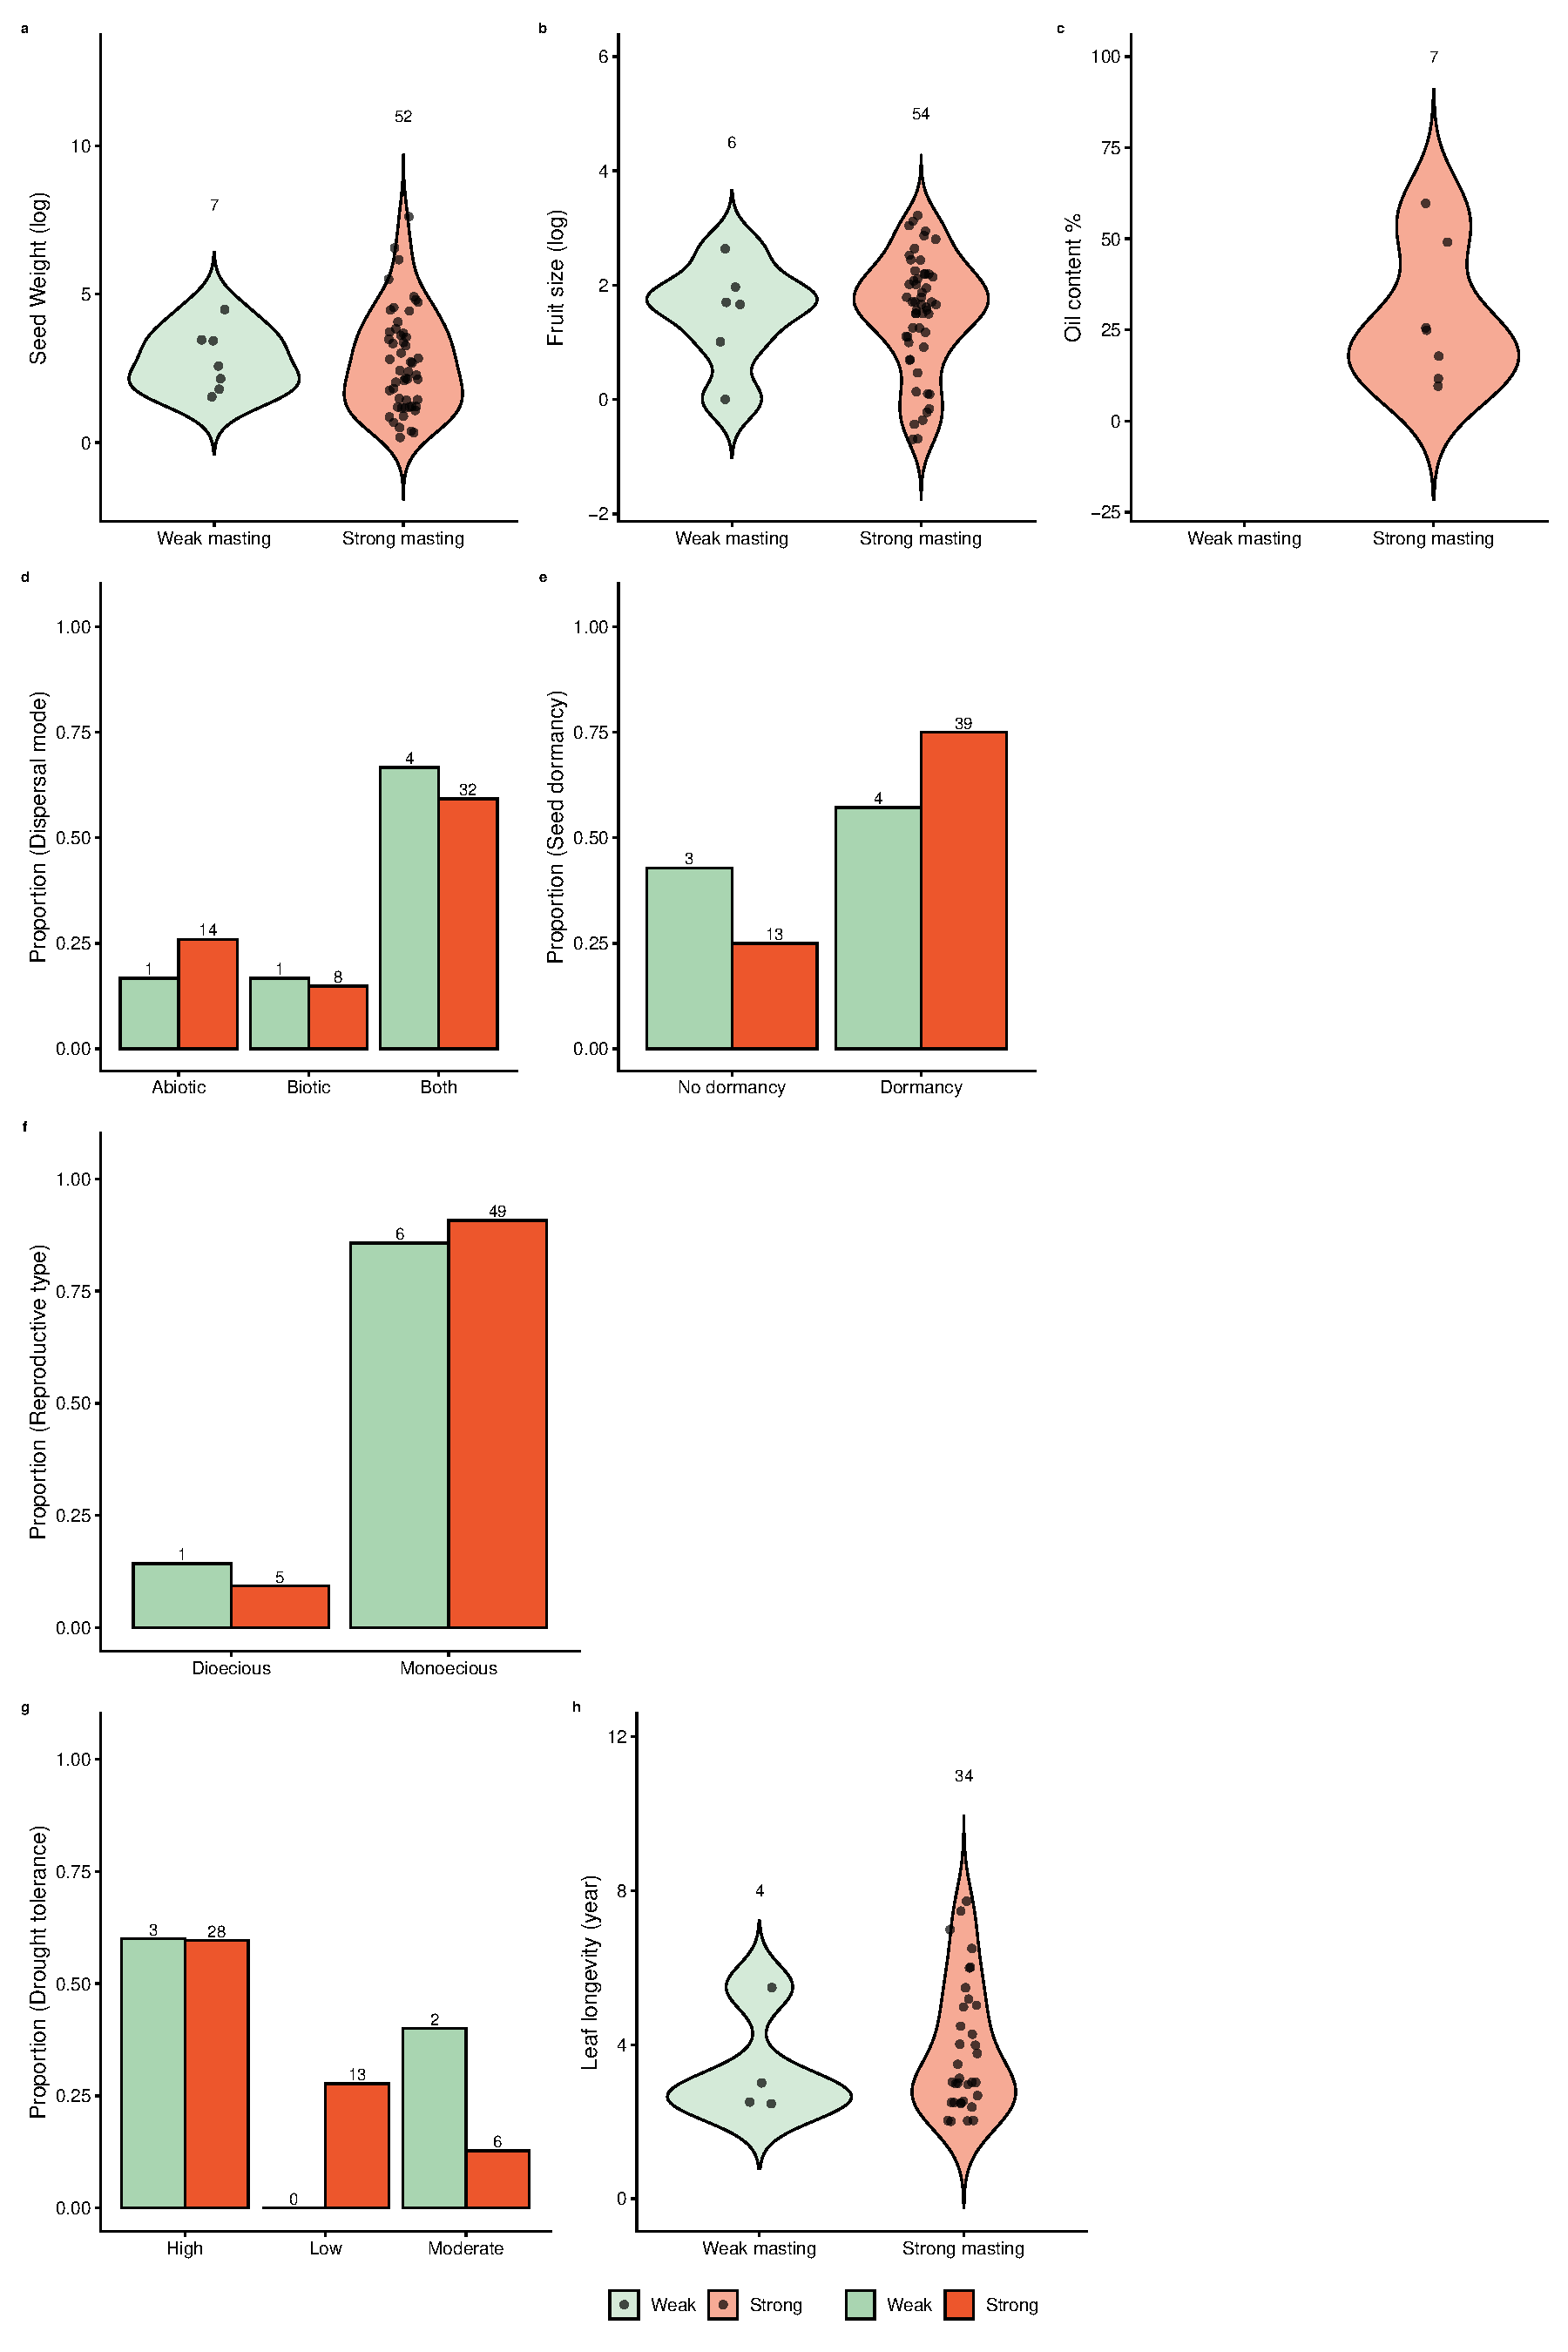
\includegraphics[width=\textwidth,height=0.8\textheight]{../output/figures/rawDataWithStatsCon.pdf}
\caption{How plant traits related to different hypotheses differ in strong masting and weak masting for gymnosperm species: We show data for traits related to the predator satiation hypothesis (a-e), pollination coupling hypothesis (f-g) and the resource matching hypothesis (h-i) as either violin plots (a-c, i) or proportional histograms (d-h) separated by species categorized as strong masting (red) or weak masting (green). We show model summaries only where significant (P-value < 0.5) and also report the model sample size (N), regression coefficient (Estimate), and phylogenetic signal parameter $\alpha$. Full model results are show in Table \ref{tab:regressiongym}.}
\label{fig:rawcon}
\end{figure}
\restoregeometry
\newpage

\begin{figure}[H]
\centering
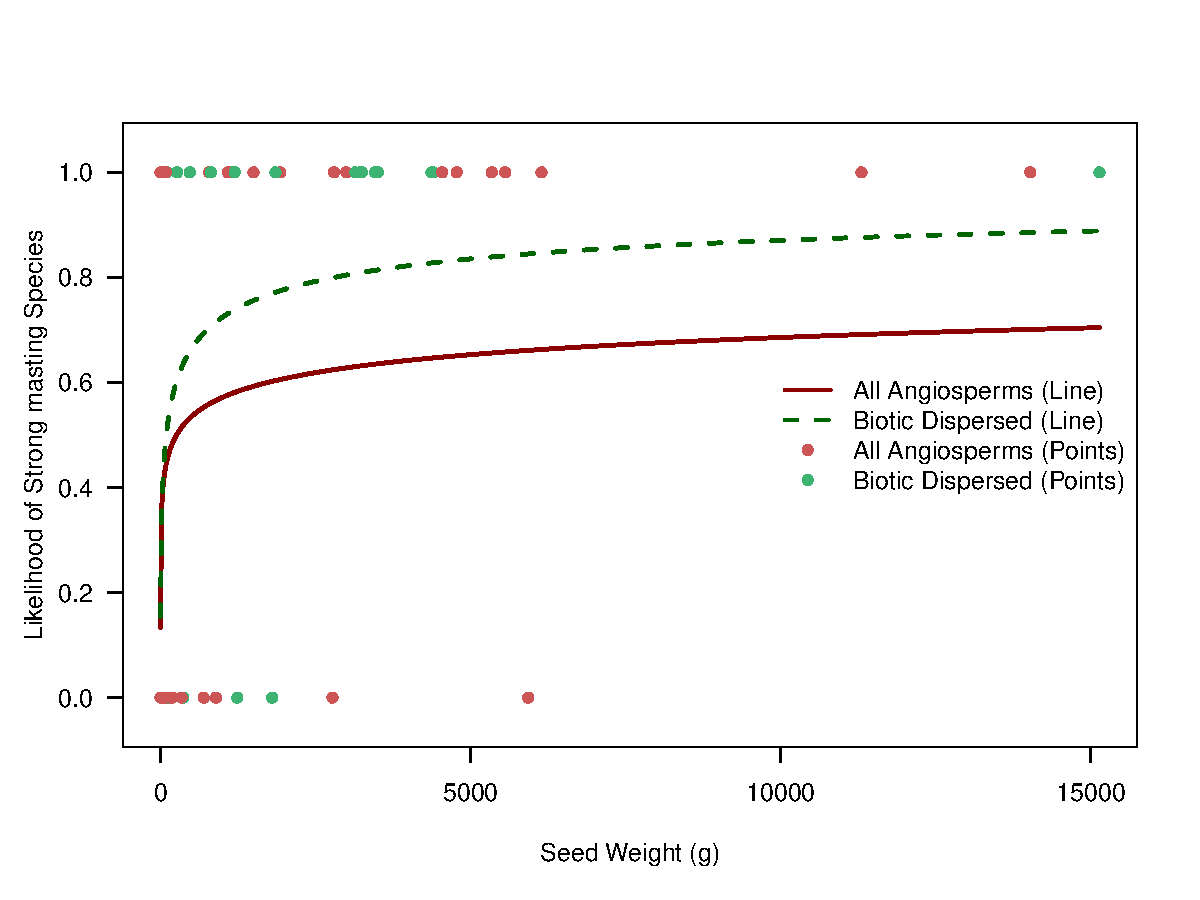
\includegraphics[width=0.8\textwidth]{../output/figures/modelFitSeedWeight.pdf}
\caption{Predicted likelihood of masting as a function of seed weight for all angiosperm species (solid red line) and the biotic-dispersed subgroup (dashed green line), estimated using phylogenetic logistic regression. Individual species observations are plotted as binary data points at 0 (weak masting) and 1 (strong masting).}
\label{fig:seedweight}
\end{figure}

\item Results for each hypothesis
\begin{enumerate}
\item Predation satiation: seed weight only with a small effect and only for angiosperm
\begin{enumerate}
\item Only seed weight is related to masting with larger seeds increasing the probability of being a strong masting species (Figure \ref{fig:rawangio}). For angiosperms only, tripling of seed weight (from a median seed weight of 90.9g to 272.7g) is predicted to increase the likelihood of strong masting from 0.45 to 0.51 (Figure \ref{fig:seedweight}).
And this increase is stronger in biotic-dispersed seed group, tripling of seed weight (from a median seed weight of 1087.15g to 3261.45g) is predicted to increase the likelihood of strong masting from 0.72 to 0.80 (Table \ref{tab:regressionseed}; Figure \ref{fig:seedweight}). 

\end{enumerate}
\item Pollination satiation: wind pollination for angiosperm
\begin{enumerate}
\item We found wind pollination is related to strong masting for angiosperm species, likelihood for wind-pollinated species is predicted to increase the likelihood of strong masting to 0.62, whereas the likelihood is 0.20 for animal-pollinated species.
of being strong masting species. Gymnosperm are all wind pollinated, and gymnosperm has a greater portion of strong masting species.
\end{enumerate}
\item Resource matching: nothing significant

\end{enumerate}
\newpage
% ------------------------------------------
\begin{figure}[H]
\centering
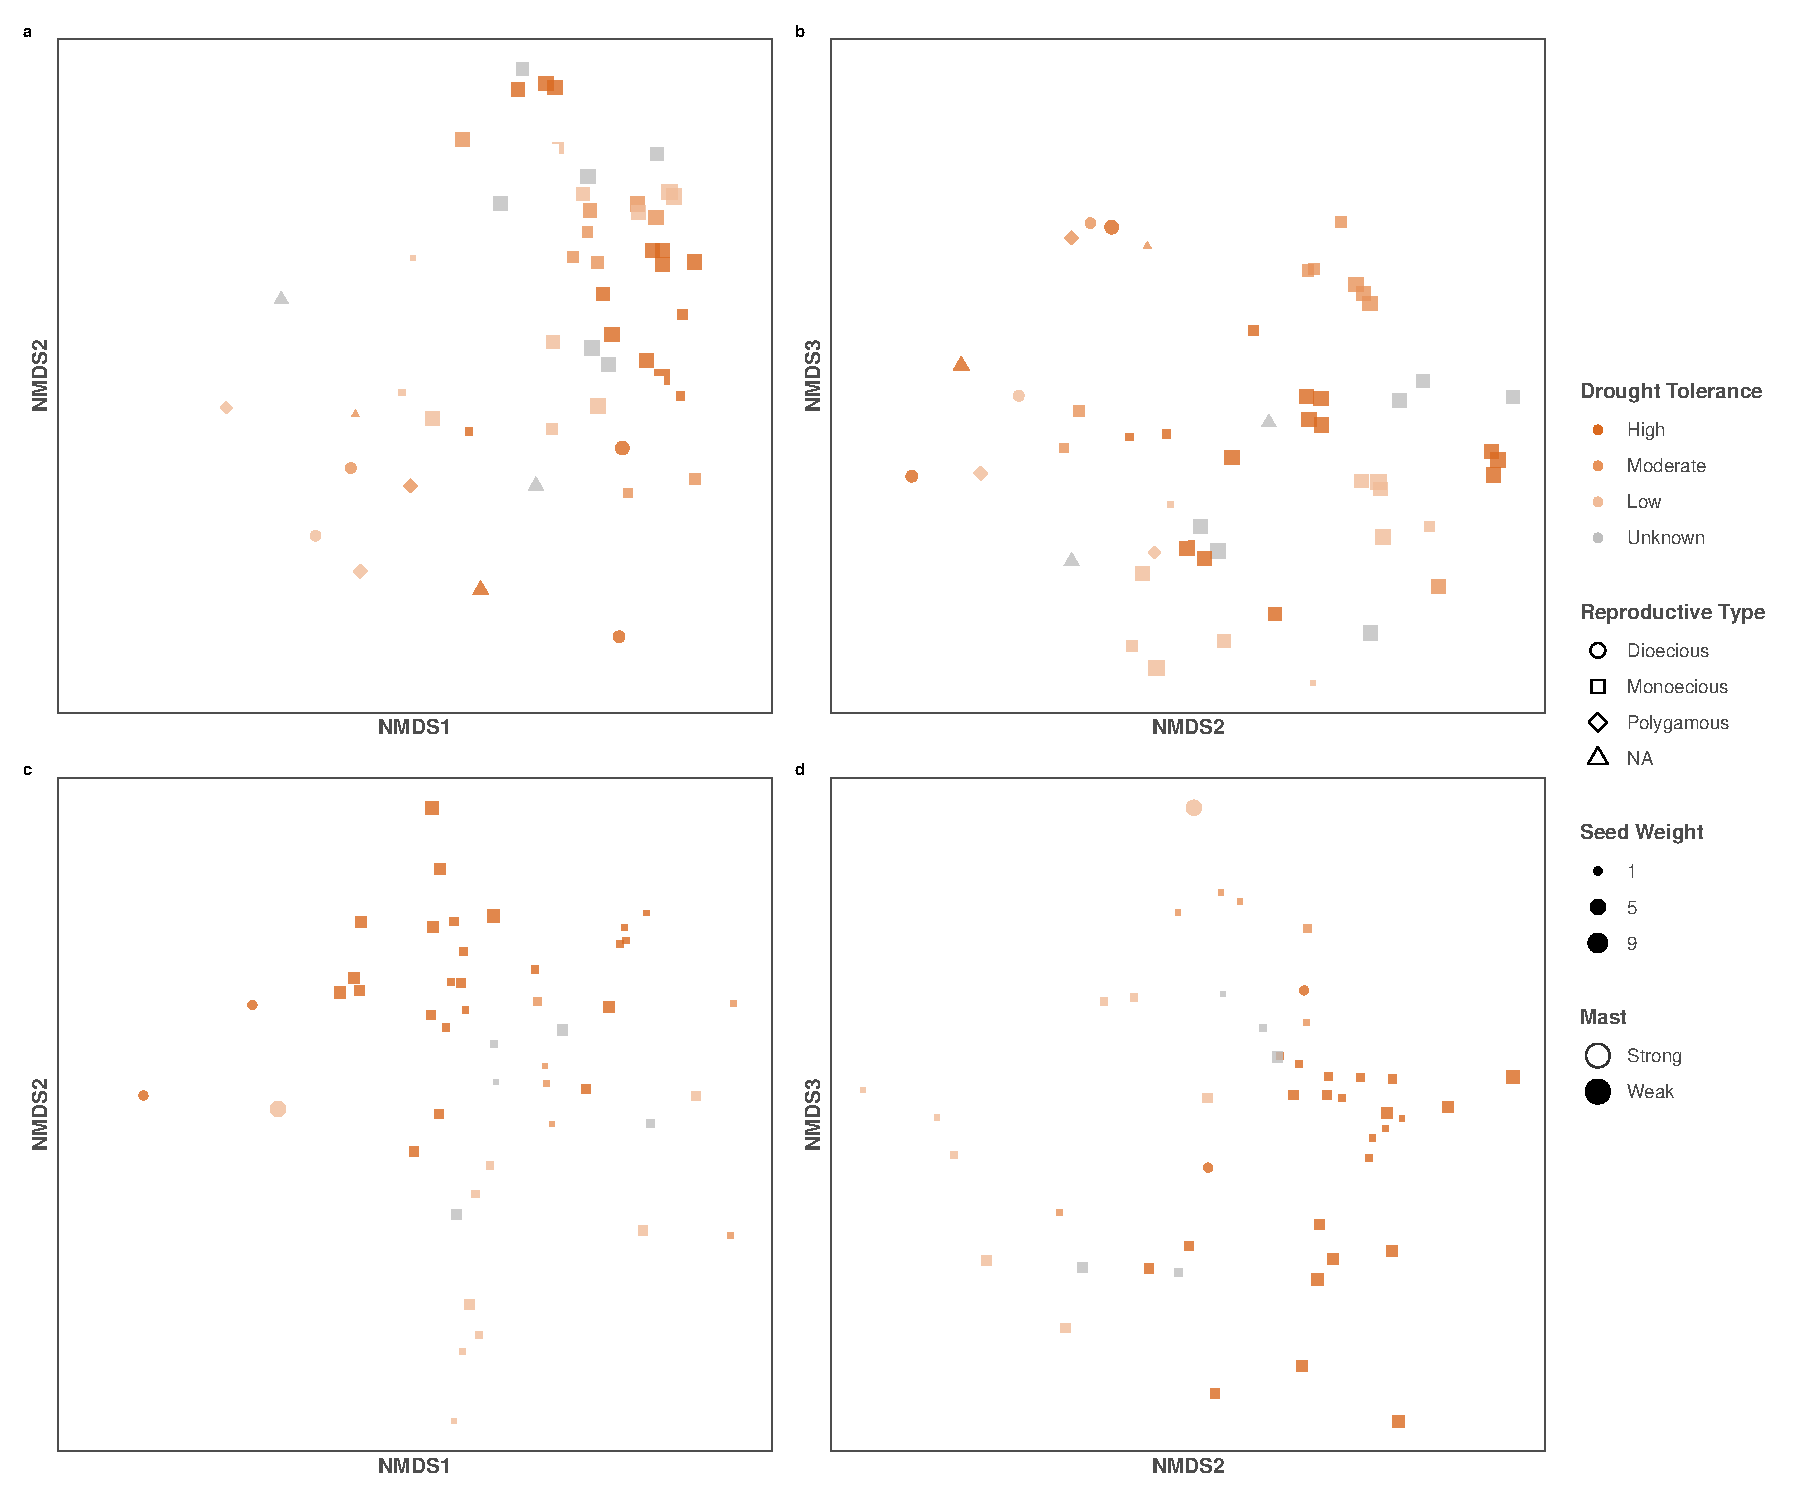
\includegraphics[width=\textwidth]{../output/figures/nmdsFinal_scalearea.pdf}
\caption{Non-metric multidimensional scaling (NMDS) of trait composition for angiosperm and gymnosperm species. Each point represents a species, with position determined by NMDS axes. Points are colored by drought tolerance, filled by strong masting or not, shaped by reproductive type, sized by seed weight. Panels are arranged as (a) angiosperm NMDS1–NMDS2, (b) angiosperm NMDS2–NMDS3, (c) gymnosperm NMDS1–NMDS2, and (d) gymnosperm NMDS2–NMDS3.}
\label{fig:nmds}
\end{figure}

\item Multidimension-NMDS
\begin{enumerate}
\item No strong trend when considering single trait, maybe because it happens in multidimensional space
\begin{enumerate} 
\item Masting is not aligned well along any axis in the NMDS analysis.
\item We do not have evidence that the combination of traits for any of the hypotheses is driving the pattern of masting.
\end{enumerate}
\end{enumerate}
% ------------------------------------------
\newgeometry{margin=1cm}
\begin{figure}[p]
\centering
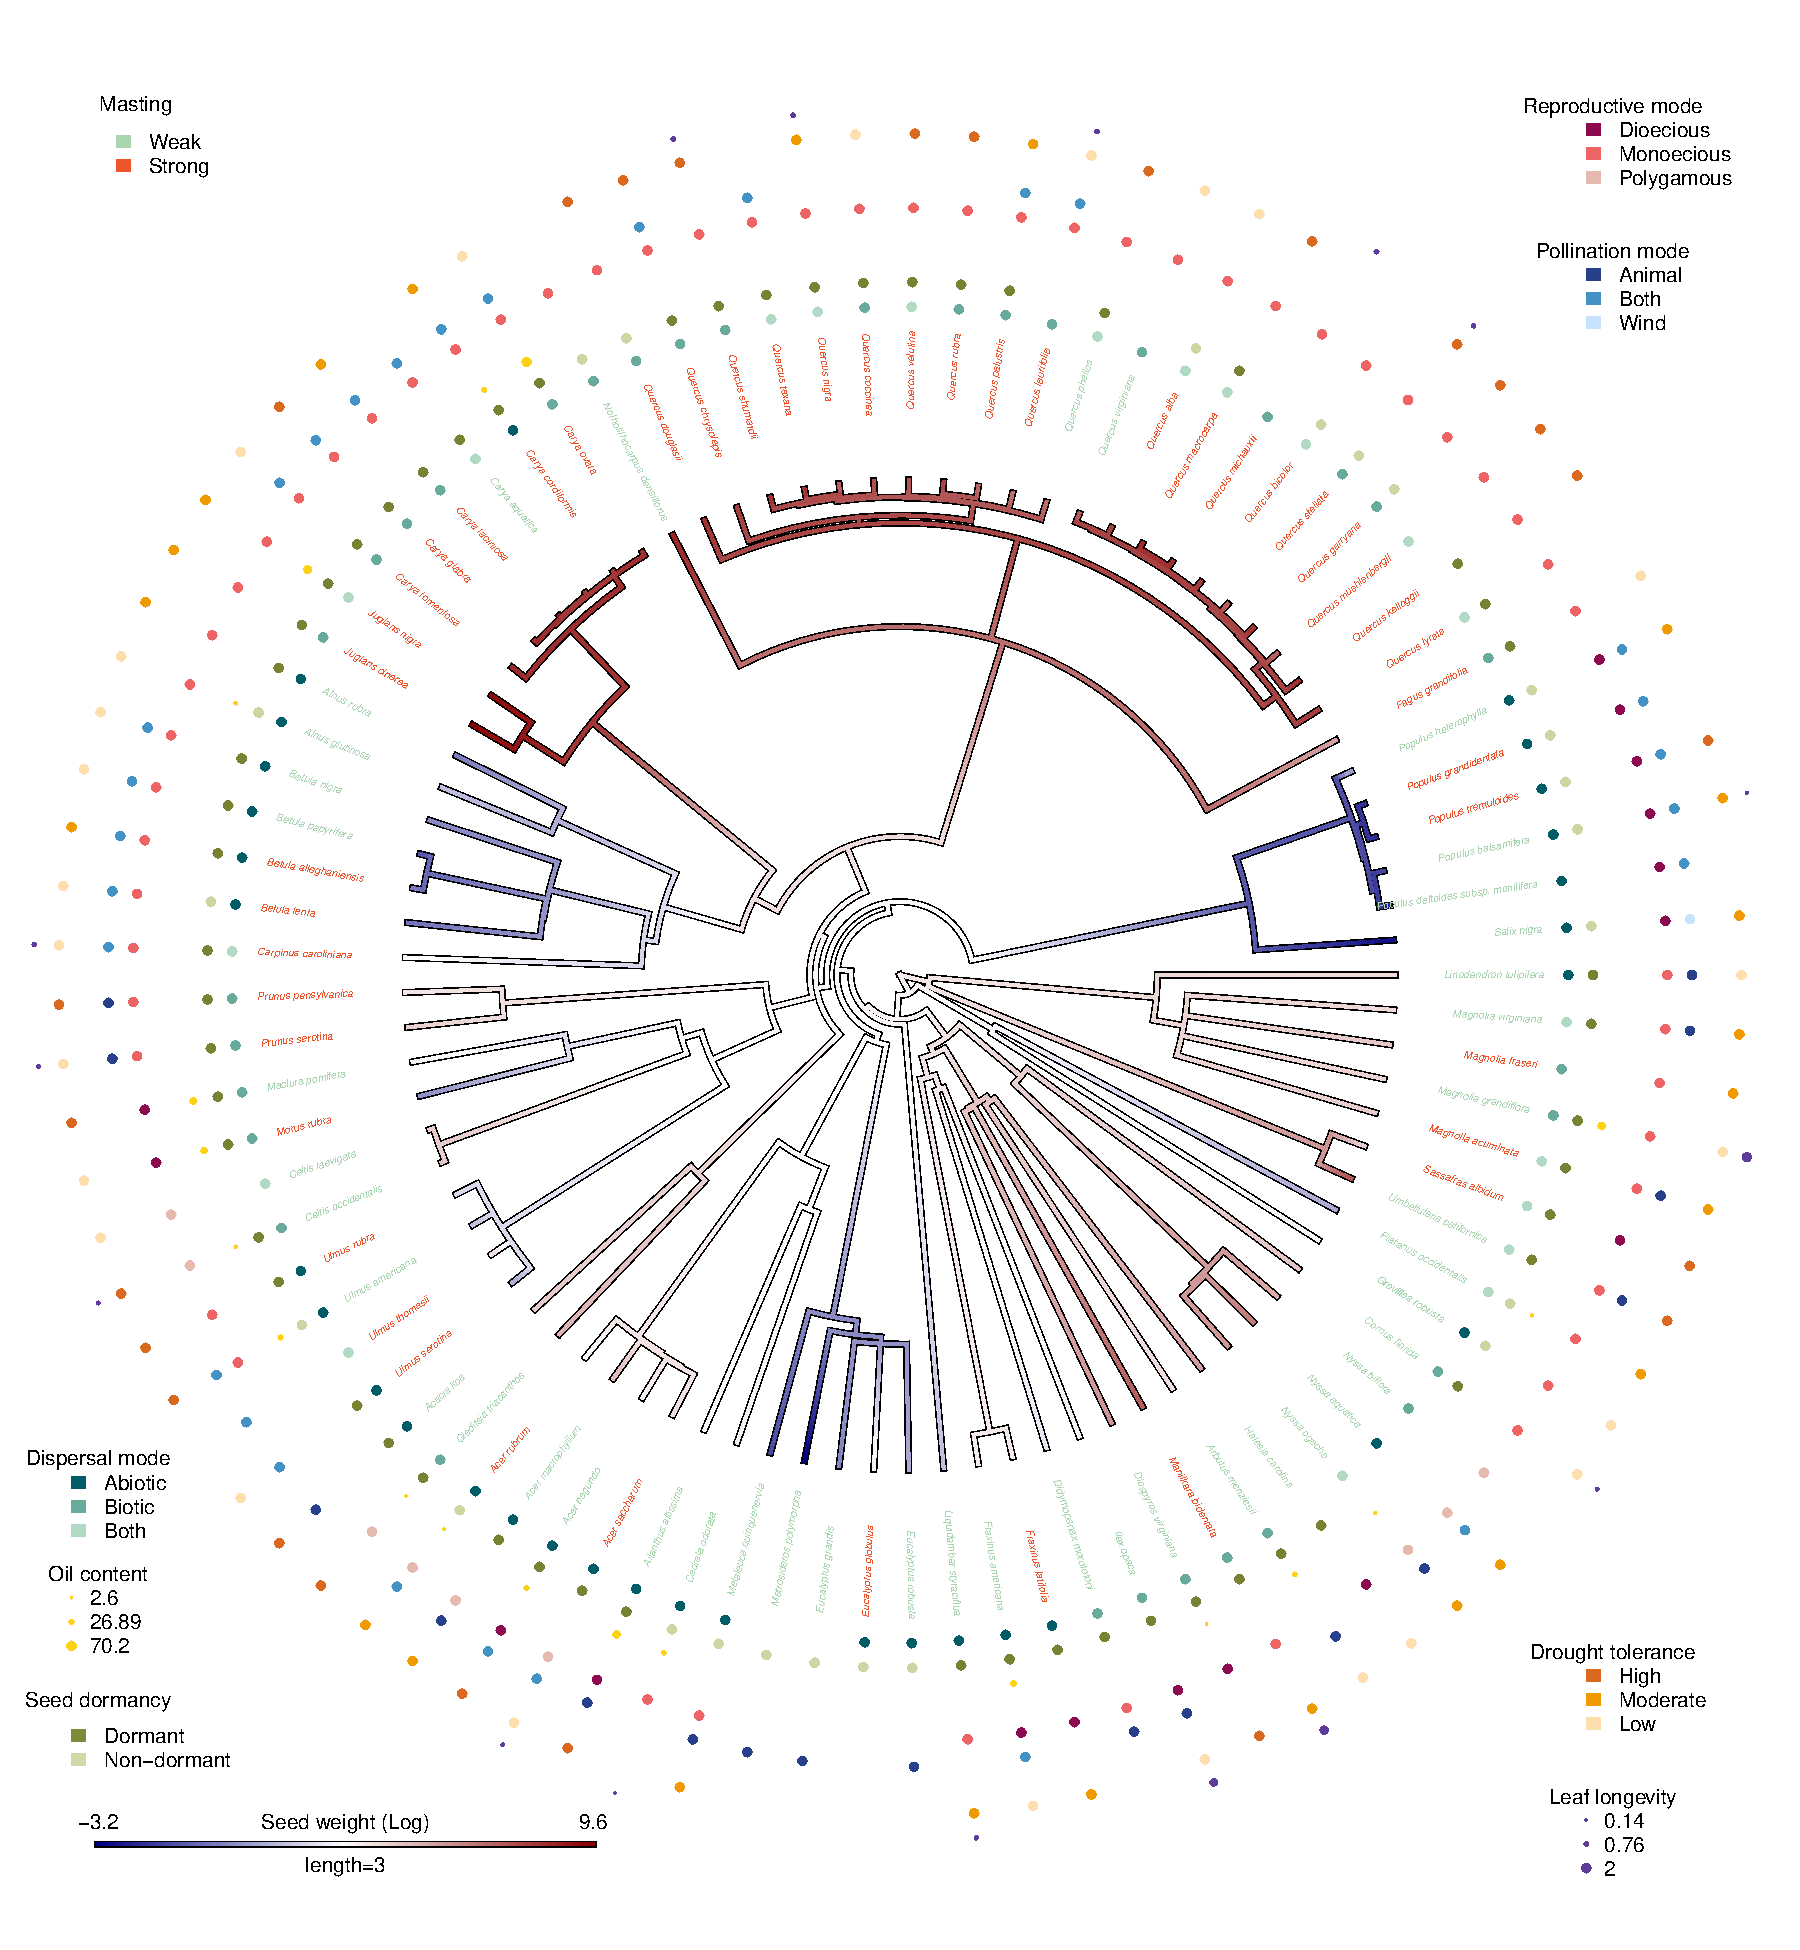
\includegraphics[width=\textwidth,height=0.9\textheight,keepaspectratio]{../output/figures/weightTree1.pdf}
\caption{Phylogenetic tree for all angioperm species included in the analysis. The color scheme of the branch is the trait value for seed weight (log). The color tip is colored by strong masting or not. The other traits are labeled after the tip labels with different color and size. We also show the predictions of relationship between traits and strong masting. We calculated the Pagel's $\lambda$ for continuous traits as well as multilevel categorical traits, and calculated D-statistic for binary traits.}
\label{fig:coneptangio}
\end{figure}
\restoregeometry
\newpage
% ------------------------------------------

\item Phylogenetic patterns
\begin{enumerate}
\item Pagel's $\lambda$ for continuous traits and multilevel categorical traits in Table \ref{tab:lambda}, D-statistic for binary traits in Table \ref{tab:dstat}.
\begin{enumerate}
\item Strong masting shows a moderate phylogenetic signal in both gymnosperms (estimated D = 0.51) and angiosperms (estimated D = 0.58) (Table \ref{tab:dstat}).
\item Seed weight has strong phylogenetic signal for both angiosperm ($\lambda$ = 0.95) and gymnosperm ($\lambda$ = 0.97). We can see the similarity in certain group in Figure \ref{fig:coneptangio} it's relatively reliable estimate. Dispersal mode, leaf longevity, pollination mode and reproductive type also showed high phylogenetic signal in Table \ref{tab:lambda}, but be cautious that $\lambda$ for categorical traits might not be accurate. 
\item Be cautious that $\lambda$ might not be comparable among traits, not only because the way $\lambda$ is calculated for continuous traits and categorical traits are different, but also because $\lambda$ might depend on the data structure when sampling is uneven, take leaf longevity as an example in Figure \ref{fig:coneptangio},leaf longevity data is sparse and nested in \textit{Quercus.} (5/16). 
\end{enumerate}

\end{enumerate}

\end{enumerate}

\clearpage
\appendix
\section{Supplementary Material}
\setcounter{table}{0}
\renewcommand{\thetable}{S\arabic{table}}

\setcounter{figure}{0}
\renewcommand{\thefigure}{S\arabic{figure}}

\begin{table}[ht]
\centering
\resizebox{\textwidth}{!}{
% latex table generated in R 4.2.3 by xtable 1.8-4 package
% Wed Jul  1 23:56:49 2026
\begin{tabular}{lllrrrrrr}
  \hline
Trait & Type & Predictor & N & Estimate & SE & P & Phylo $\alpha$ & Half-time \\ 
  \hline
Seed weight (log) & Numeric & Seed weight (log) &  89 & 0.22 & 0.09 & 0.01 & 11.34 & 0.06 \\ 
  Fruit size (log) & Numeric & Fruit size (log) &  83 & 0.00 & 0.31 & 0.99 & 28.28 & 0.02 \\ 
  Oil content (\%) & Numeric & Oil content (\%) &  19 & 0.04 & 0.03 & 0.20 & 19.22 & 0.04 \\ 
  Seed dormancy & Categorical & Dormant vs. non-dormant &  81 & 0.28 & 0.53 & 0.60 & 11.48 & 0.06 \\ 
  Dispersal mode & Categorical & Biotic vs. abiotic &  88 & 0.69 & 0.54 & 0.20 & 9.86 & 0.07 \\ 
  Dispersal mode & Categorical & Both vs. abiotic &  88 & 0.66 & 0.58 & 0.25 & 9.86 & 0.07 \\ 
  Pollination mode & Categorical & Wind vs. animal &  48 & 1.88 & 0.73 & 0.01 & 53.51 & 0.01 \\ 
  Pollination mode & Categorical & Wind vs. animal and animals &  48 & -0.25 & 2.76 & 0.93 & 53.51 & 0.01 \\ 
  Reproductive type & Categorical & Monoecious vs. dioecious &  84 & 0.93 & 0.69 & 0.18 & 13.81 & 0.05 \\ 
  Reproductive type & Categorical & Monoecious vs. polygamous &  84 & -0.13 & 0.96 & 0.89 & 13.81 & 0.05 \\ 
  Drought tolerance & Categorical & Low vs. high drought tolerance &  76 & 0.02 & 0.46 & 0.97 & 8.77 & 0.08 \\ 
  Drought tolerance & Categorical & Moderate vs. high drought tolerance &  76 & -0.31 & 0.46 & 0.50 & 8.77 & 0.08 \\ 
  Leaf longevity (years) & Numeric & Leaf longevity (years) &  16 & 0.26 & 0.95 & 0.78 & 0.90 & 0.77 \\ 
   \hline
\end{tabular}}
\caption{Phylogenetic generalized linear model results for angiosperm species. We modeled each trait separately with masting as a binary variable and traits as either categorical (Type column), where we report (Estimate column) the the difference in log-odds between a given level and its designated baseline reference level, or continuous, where we report the change in log-odds per unit increase of the predictor (Estimate column). We also report the standard error (SE), P-value (with P < 0.05 considered significant and marked with an asterisk next to the Predictor), Phylo $\alpha$, which represents the the phylogenetic signal in the residuals estimated for each trait, and the half-time (log(2)/$\alpha$), which represents the time required for the influence of ancestral states to decrease by half, where values less than 1 indicating relatively weak phylogenetic signal in the residuals.}
\label{tab:regressionangio}
\end{table}

\begin{table}[ht]
\centering
\resizebox{\textwidth}{!}{
% latex table generated in R 4.2.3 by xtable 1.8-4 package
% Wed Jul  1 23:56:49 2026
\begin{tabular}{lllrrrrrr}
  \hline
Trait & Type & Predictor & N & Estimate & SE & P & Phylo $\alpha$ & Half-time \\ 
  \hline
Seed weight (log) & Numeric & Seed weight (log) &  58 & -0.01 & 0.24 & 0.98 & 53.48 & 0.01 \\ 
  Fruit size (log) & Numeric & Fruit size (log) &  59 & 0.03 & 0.35 & 0.94 & 51.67 & 0.01 \\ 
  Seed dispersal & Categorical & Biotic vs. abiotic &  59 & -0.82 & 0.81 & 0.31 & 1.99 & 0.35 \\ 
  Seed dispersal & Categorical & Both vs. abiotic &  59 & -1.11 & 0.67 & 0.10 & 1.99 & 0.35 \\ 
  Seed dormancy & Categorical & Dormant vs. non-dormant &  58 & 0.69 & 0.70 & 0.33 & 52.49 & 0.01 \\ 
  Reproductive type & Categorical & Monoecious vs. dioecious &  60 & -1.15 & 1.02 & 0.26 & 0.91 & 0.76 \\ 
  Drought tolerance & Categorical & Low vs. high drought tolerance &  51 & 12.96 & 249.43 & 0.96 & 0.03 & 23.10 \\ 
  Drought tolerance & Categorical & Moderate vs. high drought tolerance &  51 & -0.19 & 0.57 & 0.74 & 0.03 & 23.10 \\ 
  Leaf longevity (years) & Numeric & Leaf longevity (years) &  37 & 0.14 & 0.34 & 0.67 & 54.36 & 0.01 \\ 
   \hline
\end{tabular}}
\caption{Phylogenetic generalized linear model results for gymnosperm species. We modeled each trait separately with masting as a binary variable and traits as either categorical (Type column), where we report (Estimate column) the the difference in log-odds between a given level and its designated baseline reference level, or continuous, where we report the change in log-odds per unit increase of the predictor (Estimate column). We also report the standard error (SE), P-value (with P < 0.05 considered significant and marked with an asterisk next to the Predictor), Phylo $\alpha$, which represents the the phylogenetic signal in the residuals estimated for each trait, and the half-time (log(2)/$\alpha$), which represents the time required for the influence of ancestral states to decrease by half, where values less than 1 indicating relatively weak phylogenetic signal in the residuals.}
\label{tab:regressiongym}
\end{table}

\begin{table}[ht]
\centering
\resizebox{\textwidth}{!}{
% latex table generated in R 4.2.3 by xtable 1.8-4 package
% Wed Jul  1 23:56:49 2026
\begin{tabular}{lllrrrrrr}
  \hline
Trait & Group & Predictor & N & Estimate & SE & P & Phylo $\alpha$ & Half-time \\ 
  \hline
Seed weight (log) & Biotic and both & Seed weight (log) &  53 & 0.40 & 0.15 & 0.01 & 54.57 & 0.01 \\ 
  Seed weight (log) & Abiotic & Seed weight (log) &  36 & 0.12 & 0.13 & 0.36 & 50.33 & 0.01 \\ 
   \hline
\end{tabular}}
\caption{Phylogenetic generalized linear model results for only seed weight for biotic-dispersed subgroup (both group included) and abiotic-dsipersed subgroup. We report the change in log-odds per unit increase of the predictor (Estimate column). We also report the standard error (SE), P-value (with P < 0.05 considered significant and marked with an asterisk next to the Predictor), Phylo $\alpha$, which represents the the phylogenetic signal in the residuals estimated for each trait, and the half-time (log(2)/$\alpha$), which represents the time required for the influence of ancestral states to decrease by half, where values less than 1 indicating relatively weak phylogenetic signal in the residuals.}
\label{tab:regressionseed}
\end{table}

\begin{table}[ht]
\centering

% latex table generated in R 4.2.3 by xtable 1.8-4 package
% Wed Jul  1 23:56:49 2026
\begin{tabular}{llr}
  \hline
Group & Trait & $\lambda$ \\ 
  \hline
Angiosperm & Seed weight (Log) & 0.95 \\ 
  Angiosperm & Fruit size (Log) & 0.93 \\ 
  Angiosperm & Oil content & 0.25 \\ 
  Angiosperm & Leaf longevity & 1.02 \\ 
  Angiosperm & Dispersal mode & 0.00 \\ 
  Angiosperm & Pollination mode & 1.00 \\ 
  Angiosperm & Reproductive type & 1.00 \\ 
  Angiosperm & Drought tolerance & 0.00 \\ 
  Gymnosperm & Seed weight (Log) & 0.97 \\ 
  Gymnosperm & Fruit size (Log) & 0.90 \\ 
  Gymnosperm & Oil content \% & 0.00 \\ 
  Gymnosperm & Leaf longevity & 0.90 \\ 
  Gymnosperm & Dispersal mode & 0.00 \\ 
  Gymnosperm & Drought tolerance & 1.00 \\ 
   \hline
\end{tabular}
\caption{Phylogenetic Signal (Pagel's $\lambda$) for continous traits and multi-level categorical traits. $\lambda$ = 0 indicates no phylogenetic signal, trait districuted independent of the phylogeny; 0 < $\lambda$ < 1 means moderate phylogenetic signal, trait is partially structured by the phylogeny; $\lambda$ = 1 indicates strong phylogenetic signal, trait follows Brownian motion.}
\label{tab:lambda}
\end{table}

\begin{table}[ht]
\centering
\resizebox{\textwidth}{!}{
% latex table generated in R 4.2.3 by xtable 1.8-4 package
% Wed Jul  1 23:56:49 2026
\begin{tabular}{lllll}
  \hline
Group & Trait & Estimated D & P(random) & P(Brownian) \\ 
  \hline
Angiosperm & Seed dormancy & 0.25 & 0 & 0.16 \\ 
  Angiosperm & Masting & 0.58 & 0 & 0.01 \\ 
  Gymnosperm & Masting & 0.51 & 0.02 & 0.10 \\ 
  Gymnosperm & Seed dormancy & 0.98 & 0.41 & 0 \\ 
  Gymnosperm & Reproductive type & -0.52 & 0 & 0.89 \\ 
   \hline
\end{tabular}}
\caption{Phylogenetic Signal (D-statistic) for the phylogenetic signal of binary traits, with probabilities calculated under a random phylogenetic structure and under a Brownian motion phylogenetic structure. D = 1 indicates the trait is randomly distributed across the phylogeny; D = 0 indicates the trait follows a Brownian motion model; 0 < D < 1 indivates moderate phylogenetic signal; D < 0 indicates the trait is more clumped than expected under Brownian motion; and D > 1 indicates overdispersion. P random is the p-value for the null hypothesis that the trait is randomly distributed across the phylogeny (no phylogenetic signal), and P Brownian is the p-value for the null hypothesis that the trait follows a Brownian motion model (strong phylogenetic signal). A low p-value indicates rejection of the corresponding null hypothesis.}
\label{tab:dstat}
\end{table}

\end{document}

When we know the phylogenetic results, we need to be cautious interpretating relationships between traits, it is hard to tease out traits from masting, which limits the inference)

\begin{figure}[H]
\centering
\includegraphics[width=\textwidth]{../output/figures/quercusTree.pdf}
\caption{Phylogenetic tree for all \textit{Quercus.} species, \textit{Quercus.} species included in this study is color coded.}
\label{fig:quercus}
\end{figure}
% ------------------------------------------
\subsection{Data sparsity}
\begin{enumerate}
\item Data is strongly nested in phylogeny, and data is sparse (Figure \ref{fig:coneptangio}). We have to assume the sampling is even.
\item Among all the \textit{Quercus} species with well-resolved phylogeny (268), our dataset includes only 21 species, and only two of them are weak masting species (Figure \ref{fig:quercus}).

\end {enumerate}

